%
% This document is available under the Creative Commons Attribution-ShareAlike
% License; additional terms may apply. See
%   * http://creativecommons.org/licenses/by-sa/3.0/
%   * http://creativecommons.org/licenses/by-sa/3.0/legalcode
%
% Created: 2012-07-28 10:50:36+02:00
% Main authors:
%     - Jérôme Pouiller <jezz@sysmic.org>
%

\part{Utilisation des systèmes Unix}

\begin{frame}
  \partpage
\end{frame}

\begin{frame}
  \tableofcontents[currentpart]
\end{frame}

\section{Le shell}

\begin{frame}[fragile=singleslide]{Historique}
  \begin{itemize}
  \item Mode de communication bas niveau privilègié
  \item  Lèger,  simple  à  implémenter, puissant.   Parfois  l'unique
    manière de communiquer avec le système.
  \item Le shell ``Unix'' est plus commun. Beaucoup d'autres interface
    en ligne de commande s'en inspire.
  \item Première version du shell Unix tel qu'on le connait écrite par
    Ken Thompson chez Bell Labs en 1971 (bien antérieur à Linux)
  \item Remplacé par le shell de Stephen Bourne en 1977
  \item  Par  ordre  approximatif d'apparition:  \cmd{sh},  \cmd{csh},
    \cmd{tcsh}, \cmd{ksh}, \cmd{bash}, \cmd{zsh}, \cmd{ash}
  \item Normalisé par la Posix 2 en 1992
  \item Fonctionne de manière plus  ou moins identique sur tous les OS
    (Linux, Androïd, iOS, Windows/Cygwin, etc...)
  \item On peut faire beaucoup de chose avec la ligne de commande
  \item Il  est possible de  faire des script  en shell. Il  arrive ce
    soir le seul langage de script disponible sur le système.
  \end{itemize}
\end{frame}

\subsection{Bases}

\begin{frame}[fragile=singleslide]{Bases de shell}
  \begin{itemize}
  \item Lancer une commande (= lancer un programme)
    \begin{lstlisting}
$ ls
    \end{lstlisting} %$
  \item Séparation des arguments par des espaces
    \begin{lstlisting}
$ mkdir dir1 dir2
    \end{lstlisting} %$
  \item Conséquence: les espaces sont des caractères spéciaux en shell
  \item  Les  arguments sont  recus  par  le  programme par  les  deux
    arguments \c{argc} et \c{argv}
  \item  Remarque: certaines commandes  ont un  comportement différent
    suivant \c{argv[0]} (exemple: \c{test} et \c{[})
  \end{itemize}
\end{frame}

\begin{frame}[fragile=singleslide]{Convention}
  Par convention,  nous préfixons dans ces slides  les commandes shell
  par :
  \begin{itemize}
  \item  \c{$}  pour les  commandes  à  éxecuter par  l'utilisateur
    normal
  \item \c{\%} pour les commande à executer par root
  \item \c{>} pour les commandes non-shell
  \end{itemize}
\end{frame}

\begin{frame}[fragile=singleslide]{Les argument optionnels}
  \begin{itemize}
  \item Souvent les arguments optionnels commence par ``\c{-}''
  \item Les options peuvent avoir des arguments
  \item Il existe des options longues commencant par ``\c{--}''
    \begin{lstlisting}
$ ls --all
$ ls --sort=time
$ ls --sort time
    \end{lstlisting}
  \item  ... et des  options courte  tenant sur  un seul  caractère et
    commencant  par un  simple  ``\c{-}'' (attention  tout  de même  aux
    exceptions)
    \begin{lstlisting}
$ ls -l -a
$ ls
    \end{lstlisting}
  \end{itemize}
\end{frame}

\begin{frame}[fragile=singleslide]{Les argument optionnels}
  \begin{itemize}
  \item Il est possible de concaténer les option courtes
    \begin{lstlisting}
$ ls -la
    \end{lstlisting} %$
  \item Les options ne  sont \emph{normalement} pas dépendante de leur
    emplacement
    \begin{lstlisting}
$ ls -la
    \end{lstlisting} %$
  \item Ce  principe est normalisé car toutes  ces commandes utilisent
    la fonction Posix \man{getopt(3)} (mais rien ne le garanti)
  \end{itemize}
\end{frame}

\begin{frame}[fragile=singleslide]{La documentation}
  \begin{itemize}
  \item  \cmd{man  COMMAND} permet  d'accèder  à  la documentation  de
    \c{COMMAND}
  \item  Les  pages  de  man  sont  divisée  en  9  sections
  \item D'après \man{man(1)}):
    \begin{enumerate}
    \item Executable programs or shell commands
    \item System calls (functions provided by the kernel)
    \item Library calls (functions within program libraries)
    \item Special files (usually found in /dev)
    \item File formats and conventions (e.g. \file{/etc/passwd})
    \item Games
    \item  Miscellaneous (including  macro packages  and conventions),
      e.g.  \man{man(7)}, \man{groff(7)}
    \item System administration commands (usually only for root)
    \item Kernel routines [Non standard]
    \end{enumerate}
  \end{itemize}
\end{frame}

\begin{frame}[fragile=singleslide]{La documentation}
  \begin{itemize}
  \item Une même entrée peut  être présente dans plusieurs section, il
    possible de préciser la section en la placant en argument avant la
    commande:
    \begin{lstlisting}
$ man read
$ man 2 read
    \end{lstlisting}
  \item Les références des pages de  man sont donnés avec le numéro de
    section entre parenthèses.  Ainsi, \man{wait(2)} signifie que vous
    pouvez   accéder    à   la   documentation    avec   la   commande
    \cmd{man 2 wait}
  \item \cmd{man -l}  permet d'afficher un fichier \emph{local}
  \item \c{man man} pour plus d'information
  \end{itemize}
\end{frame}

\begin{frame}[fragile=singleslide]{Les chemins}
  Il est possible d'utiliser des chemins:
  \begin{itemize}
  \item absolus, commencant par un \c{/}
    \begin{lstlisting}
$ mkdir /tmp/tete
    \end{lstlisting}
  \item relatifs, commencant par un autre caractère
    \begin{lstlisting}
$ mkdir tmp/titi
    \end{lstlisting}
  \end{itemize}
  Les  chemins  relatifs, s'interprête  à  partir du  \emph{répertoire
    courant}  (lié au  processus actuel  et hérité  par  les processus
  fils).
  \begin{itemize}
  \item \cmd{pwd} affiche le répertoire courant
  \item \cmd{cd} modifie le répertoire courant
  \end{itemize}
\end{frame}

\begin{frame}[fragile=singleslide]{Les chemins}
  \begin{itemize}
  \item Dans un chemin, ``\c{.}'' correspond au répertoire courant
  \item ... \cmd{mkdir foo} est identique à \cmd{mkdir ././foo}
  \item ``\cmd{..}'' correspond au répertoire parent
  \item  Beaucoup de  commandes  prennant en  parametre un  répertoire
    utilise le  répertoire courant si le paramètre  n'est pas spécifié
    (ex: \cmd{ls})
  \item  cf. \man{path\_resolution(7)}
  \end{itemize}
  Note: Les fichiers commencant  par '\c{.}' sont considérés comme des
  fichiers cachés
\end{frame}

\begin{frame}[fragile=singleslide]{Le PATH}
  % TODO: A replacer autre part
  % Normalisées par Posix, plus  ou moins regroupée dans un projet
  %  nommé coreutils
  \begin{itemize}
  \item Une commande est recherchée dans la variable \c{$PATH}
  \item  Par  défaut,   \c{$PATH}  contient  \file{/bin}  \file{/sbin}
    \file{/usr/bin} et \file{/usr/sbin}
  \item  Si  on  spécifie  le  chemin (la  commande  contient  \c{/}),
    \c{$PATH} n'est pas utilisé
  \item  Par conséquent, pour  lancer une  binaire dans  le répertoire
    courant: \cmd{./a.out}
  \item Ajouter \c{.} dans \c{$PATH} est une mauvaise pratique
  \item Mécanisme géré par la fonction Posix \man{execvpe(3)}
  \end{itemize}
\end{frame}

\begin{frame}[fragile=singleslide]{Le contenu des fichiers}
  \begin{itemize}
    \item Ne pas oublier qu'un fichier n'est qu'un vecteur d'octet
    \item Les fichiers \emph{texte} ont simplement la particularité de
      n'avoir que  des octets supérieurs  à \c{0x20} (et les  octets >
      \c{0x7F} s'interprètent  suivant la région)  (cf. \man{ascii(7)}
      et \man{charsets(7)})
    \item Le principe de ``type'' de fichier est finalement assez flou.
    \item \man{file(1)} permet de repérer le format des fichier
    \item L'utilisation d'une norme de nommage ou d'une extention peut
      aussi  aider, mais  ca  n'est  pas une  pratique  native sur  la
      plupart des OS.
    \end{itemize}
\end{frame}

\begin{frame}[fragile=singleslide]{Les file descriptor}
  \begin{itemize}
  \item  Lorsqu'un programme  souhaite  accèder à  un  fichier, il  va
    utiliser  la  fonction Posix  \man{open(3)}  qui  lui retourne  un
    nombre   appellé  \emph{file  descriptor}   (\emph{descripteur  de
      fichier}).
  \item Il s'agit d'un identifiant pour une structure dans l'OS.
  \item  Le file  descriptor peut  être passé  à d'autre  fonctions du
    système comme \man{read(3)} ou \man{write(3)}.
  \item  Nous   verrons  plus  tard  que  le   concept  de  \emph{file
      descriptor} va plus loin
  \item  Les couche basses  de l'OS  ouvre automaitquement  trois file
    descriptor lors qu'un programme est lancé:
    \begin{itemize}
    \item    Entrée    standard     (numéro    0),    accessible    en
      lecture. Normalement reliée au clavier.
    \item    Sortie    standard     (numéro    1),    accessible    en
      écriture. Normalement reliée à l'écran
    \item    Sortie    d'erreur     (numéro    2),    accéssible    en
      écriture. Normalement reliée à l'écran
    \end{itemize}
  \end{itemize}
\end{frame}

\begin{frame}[fragile=singleslide]{Les redirections}
  Il est possible de demander au shell de rediriger les entrée est les
  sortie d'une commande avec les metacaractère \c{<} \c{>} et \c{|}:
  \begin{itemize}
  \item Commande standard:
    \begin{lstlisting}
$ echo foo
    \end{lstlisting}
  \item Sortie standard vers un fichier
    \begin{lstlisting}
$ echo foo > file
    \end{lstlisting}
  \item Un fichier vers l'entrée standard
    \begin{lstlisting}
$ cat -n < file
    \end{lstlisting} %$
  \item Sortie d'erreur vers un fichier
    \begin{lstlisting}
$ ls toto 2> file
    \end{lstlisting} %$
  \end{itemize}
\end{frame}

\begin{frame}[fragile=singleslide]{Les Redirections}
  \begin{itemize}
  \item Sortie standard d'une commande vers l'entrée d'une autre
    \begin{lstlisting}
$ echo bar foo | wc
    \end{lstlisting}
  \item Couplage des redirections
    \begin{lstlisting}
$ cat -n < file1 | wc > file3
    \end{lstlisting} %$
  \item L'espace n'est pas obligatoire et les redirections ne sont pas
    forcement à la fin de la ligne
    \begin{lstlisting}
$ >file2 cat<file1 -n
    \end{lstlisting} %$
  \item Certaine commande detecte que la sortie est redirigée et se
    comporte différement
    \begin{lstlisting}
$ ls
$ ls | cat -n
$ ls > file
    \end{lstlisting}
  \end{itemize}
\end{frame}

\subsection{Les variables}

\begin{frame}[fragile=singleslide]{Les variables locales}
  \begin{itemize}
  \item Affectation:
    \begin{lstlisting}
$ FOO=foo
    \end{lstlisting}
  \item  Rappel: en  shell, l'espace  est un  métacaractère  donc, ces
    commandes ne fonctionnent pas:
    \begin{lstlisting}
$ FOO = foo
$ FOO=foo bar
    \end{lstlisting}
  \item Il est possible de les concaténer avec \c{+=}
    \begin{lstlisting}
$ FOO+=bar
    \end{lstlisting}
  \end{itemize}
\end{frame}

\begin{frame}[fragile=singleslide]{Les variables locales}
  La  syntaxe  \c{$\{VAR\}}  permet  de  récupérer  le  contenu  d'une
  variable.  Elle peut-être abbregée  \c{$VAR} si elle est suivit d'un
  caractère non-alpha-numérique
  \begin{lstlisting}
$ echo ${FOO}
$ echo $FOO
$ echo ${FOO}_bar $FOO_bar
  \end{lstlisting}
  Sous zsh, \c{vared VAR} permet d'éditer intéractivement une variable
\end{frame}

\begin{frame}[fragile=singleslide]{Les variables d'environnement}
  \begin{itemize}
  \item   Tous  les   processus  possède   un  ensemble   de  variable
    d'envionement.
  \item  Elle   se  trouvent   dans  l'espace  mémoire   du  processus
    (cf. \man{environ(7)})
  \item   On   y    accéder   facilement   avec   \man{getenv(3)}   et
    \man{setenv(3)}
  \item  Par défaut,  un processus  hérite de  l'environnement  de son
    parent (cf. \man{exev(3)})
  \item  Un programme peut  modifier son  comportement en  fonction du
    contenu de l'environnement
  \item \cmd{export} liste les variable d'environnement
  \item \cmd{export  VAR} transforme  une variable locale  en variable
    d'environement, ou instancie la variable
  \end{itemize}
\end{frame}

\begin{frame}[fragile=singleslide]{Les variables d'environnement}
  \begin{itemize}
  \item  Il est  possible de  lancer  une commande  avec une  varibale
    d'envionnement particulière:
    \begin{lstlisting}
$ LANG=fr_FR.utf8 ls non-existant
ls: impossible d'accéder à  non-existant: Aucun fichier ou dossier de ce type
    \end{lstlisting}
  \item  ... ou  en utilisant  la commande  \c{env}, qui  possède plus
    d'options
    \begin{lstlisting}
$ env LANG=fr_FR.utf8 ls non-existant
ls: impossible d'accéder à  non-existant: Aucun fichier ou dossier de ce type
    \end{lstlisting}
  \item Les  variables d'environnement auront  un impact sur  tous les
    sous-processus lancés
  \item Leur  fonctionnement est  très différent des  variables shell,
    mais elle sont gérée avec la même syntaxe
  \end{itemize}
\end{frame}

\begin{frame}[fragile=singleslide]{Les variables d'environnement}
  Les variables d'environnement importantes:
  \begin{itemize}
  \item \c{PATH}: les chemins ou les commandes doivent être recherchée
  \item   \c{LANG},    \c{LOCALE}   et   \c{LC_*}:    les   information
    d'internationnalisation
  \item  \c{DISPLAY}:  l'addresse  du  serveur  d'affichage  pour  les
    commande graphique
  \item \c{TERM}: le type de  terminal utilisé (nécessaire pour le bon
    affichage des couleur et des outils fenetrés)
  \item \c{LS_COLOR}:  contient la  configuration de coloration  de la
    command \c{ls --color}
  \item \c{PAGER}, \c{EDITOR}, \c{BROWSER}:  Les outils à utilisé pour
    visualiser, éditer et aller sur le web.
  \end{itemize}
\end{frame}

\begin{frame}[fragile=singleslide]{La syntaxe évoluée des variable}
  La syntax des variables peut être plus évoluée:
  \begin{itemize}
  \item  \c{$\{VAR#foo\}} ou  \c{$\{VAR/foo/bar\}} pour  effectuer des
    modifcation sur les variables
  \item \c{VAR=( a b c )} pour affecter un tableau
  \item \c{$\{VAR[3]\}} pour lire une value dans un tableau
  \item  Dans un  script  ou  dans une  fonction  shell, les  variable
    \c{$1}, \c{$2}, ... correspondent  aux arguments. \c{$*} et \c{$@}
    signifient ``Tous les arguments''
  \item \c{$((21 * 2))} et \c{$[43 - 1]} sont remplacé par le résultat
    de l'expression aritthmétique
  \item  \c{$(echo toto)}  ou \c{`echo  toto`} sont  remplacés  par le
    résultat de la commande \c{echo toto}.
  \end{itemize}
\end{frame}

\begin{frame}[fragile=singleslide]{L'escaping}
  Sans surprise, il est  possible d'échapper un caractère spécial avec
  ``\c{\\}''
  \begin{lstlisting}
$ perl -e print\ \"Hello\ World\\n\"\;
  \end{lstlisting}
  Il est aussi possible de \emph{quoter} un argument
  \begin{itemize}
  \item Le \emph{double quote} \c{"} echappe la plupart des caractères
    sauf les variable et le \c{"} de fin:
    \begin{lstlisting}
$ perl -e "print \"Hello World\n\";"
    \end{lstlisting}
  \item Le \emph{simple quote} \c{'} escape tous les caractère sauf le
    caractère \c{'} de fin. Il ne peux pas être echappé:
    \begin{lstlisting}
$ perl -e 'print "Hello World\n";'
    \end{lstlisting}
  \item  Le \emph{backquote}  n'est pas  un quoting,  il  correspond à
    \c{$()}
  \end{itemize}
\end{frame}

\subsection{Les patterns}

\begin{frame}[fragile=singleslide]{Le globbing}
  \begin{itemize}
  \item Langage composé de trois metacaractères:
    \begin{itemize}
    \item \c{\?}:n'importe quel caractère
    \item \c{*}: n'importe quel caractère répété 0 ou plusieurs fois
    \item  \c{[]}: N'importe  lequel des  caractère compris  entre les
      crochets
    \end{itemize}
  \item  Le shell  essaie  de faire  correspondre  tous les  arguments
    contenant ces metacaractère avec les fichier du répertoire courant
  \item ...  il remplace ensuite le  pattern par la  liste des fichier
    correspondants
    \begin{lstlisting}
$ wc -l *.c
    \end{lstlisting}
  \item Les commandes recoivent la liste des fichiers en argument, pas
    le pattern
  \item ... deux exception notables: \c{find -name} et \c{dpkg -l}. Il
    est necessaire de correctement les quoter pour que le pattern soit
    effectivement transmis à la commande
  \end{itemize}
\end{frame}

\begin{frame}[fragile=singleslide]{Les expressions régulières}
  \begin{itemize}
  \item Ressemble de loin au globbing
  \item Plus de metacaractères:
    \begin{itemize}
    \item \c{.}: N'importe quel caractère
    \item \c{[]}:  N'importe lequel  des caractères contenu  entre les
      crochets
    \item \c{*} Le caractère précédants répété 0 ou plusieurs fois
    \item \c{+} Le caractère précédant répété 1 ou plusieurs fois
    \item \c{\{X,Y\}} Le caractère précédant répété entre X et Y fois.
    \item  \c{()} Mémorise  un  groupe qui  peut  être référencé  avec
      \c{\\X}
    \item \c{^} \c{$} Début et fin de ligne
    \end{itemize}
  \item ... voir \man{regex(7)} pour la spécifiction complète
  \end{itemize}
  Ainsi:
  \begin{itemize}
  \item \c{^a.*b.*$} matche avec \c{a123b45}
  \item \c{^a(.)*b\1$} matche avec \c{a1111b1}
  \end{itemize}
\end{frame}

\begin{frame}[fragile=singleslide]{Les expressions régulières}
  \begin{columns}
    \begin{column}{6cm}
      \begin{itemize}
      \item D'un  point de vu  formel, les expressions  régulières peuvent
        décrire des grammaires régulières (de Type 3 dans la hiérarchie de
        Chompsky)
      \item Il  est possible de  démontrer qu'il est existe  une bijection
        entre  l'ensemble  des  expressions  régulière et  l'ensemble  des
        automates à état fini
      \item A titre de comparaison, Bison est un outils capable d'exprimer
        des grammaires de Type 2 (dite \emph{context-free})
      \end{itemize}
    \end{column}
    \begin{column}{4cm}
      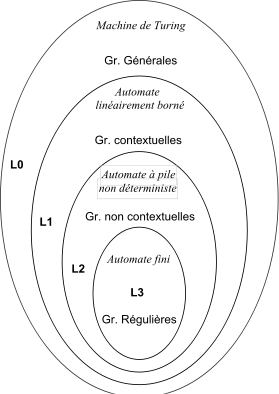
\includegraphics[height=7cm]{pics/HierarchieChomsky}
    \end{column}
  \end{columns}
\end{frame}

\begin{frame}[fragile=singleslide]{Les expressions régulières}
  Les deux implémentations de  moteur d'expression regulières les plus
  répandues  sont celles  de  GNU (Gnu  Regular Expression  Processor,
  \man(grep(1))) et de Perl.
  \begin{lstlisting}
$ echo a123b45 | grep -E '^a.*b.*$'
a123b45
$ echo a1111b1 | perl -ne 'print if /^a(.)*b\1$/;'
a1111b1
  \end{lstlisting}
  \begin{itemize}
  \item Il  peut exister des différences entre  les implémentations de
    Perl et de \cmd{grep}
  \item  Beaucoup de  commande  prennent des  expression régulière  en
    entrée. Attention à  ce qu'elle ne soit pas  interprétées comme du
    globbing par le shell
  \item Les expressions régulières, c'est bon, mangez-en.
    % TODO  faire un slide entier  d'exemple d'expressions régulières,
    % avec matching de fonction C, d'IP, etc...
  \end{itemize}
\end{frame}

\begin{frame}[fragile=singleslide]{Outils dérivés}
  Quelques outils pour travailler avec les expression régulières
  \begin{itemize}
  \item  \cmd{ed}, \cmd{grep},  \cmd{sed}, \cmd{awk},  \cmd{perl -pe}:
    Outils de traitement de texte automatique
  \item \cmd{ed}, \cmd{ex}, \cmd{vi}, \cmd{vim}: Editeurs de texte
  \end{itemize}
\end{frame}

\subsection{Quelques sujets plus avancés}

\begin{frame}[fragile=singleslide]{Le terminal}
  \begin{itemize}
  \item Lourd historique
  \item  Il existe(ait)  énormément de  terminaux  différents. Chaque
    terminal à ses spécificitées:
    \begin{itemize}
    \item caractère permettant le retour à la ligne,
    \item possibilité de déplacer le curseur,
    \item possibilité de souligner,
    \item de metter des caractères en gras,
    \item terminaux en couleur,
    \item  séquence retournée  par les  touches  spéciales (backspace,
      delete, flèche, touches de fonction, composition de touches,...)
    \end{itemize}
  \item Le minitel est(était) un terminal compatible VT102
  \end{itemize}
\end{frame}

\begin{frame}[fragile=singleslide]{Le terminal}
  \begin{itemize}
  \item   Les   terminaux  virtuel   choisissent   quelle  norme   ils
    implémentent (il peuvent en faire une nouvelle)
  \item La variable d'environnement \c{$TERM} indique aux commandes le
    type de terminal. De nos jours, la valeur \c{xterm} est de loin la
    plus répandue.
  \item \c{<Ctrl+V>} permet d'afficher la séquence de touche recue par
    le shell sans l'interpréter
  \item Les couleurs  se font avec des séquence  d'échappement plus ou
    moins  standardisée (Norme ECMA-48):  \c{\x1B[32m} pour  le rouge,
    etc...  (cf \man{console\_codes(4)})
  \item  La bibliothèque  \c{readline}, très  largement  utilisée gère
    tout  cet aspect.   \c{readline} inclut  une base  de  données des
    fonctionnalités de tous les terminaux existants
  \item Exception notable à  cette norme: Les systèmes d'exploitations
    de Microsoft  (il est possible  de commander le terminal  avec des
    appels systèmes)
  \end{itemize}
\end{frame}

\begin{frame}[fragile=singleslide]{Jobs control}
  \begin{itemize}
  \item  Il est  possible de  travailler avec  plusieurs  commandes en
    parallèles
  \item \c{<CTRL+Z>}  suspend la commande courante. En  fait, c'est le
    noyau qui transforme cette combinaison  de touche en signal et qui
    suspend le programme si celui-ci lui permet.
  \item    \c{fg}   continue   l'éxecution    de   la    commande   en
    \emph{foreground}
  \item    \c{bg}   continue   l'éxecution    de   la    commande   en
    \emph{background}
  \item  Il  est  possible  de  lancer  une  commande  directement  en
    backgound en la terminant pas \c{&}
  \item \c{jobs} liste les jobs en cours d'éxection
  \end{itemize}
  \begin{lstlisting}
$ cp -r bigdir newdir
<CTRL+Z>
$ sleep 100 &
$ jobs
[1]  - suspended  cp -r bigdir newdir
[2]  + running    sleep 100
  \end{lstlisting}
\end{frame}

\begin{frame}[fragile=singleslide]{Ecrire des scripts}
  \begin{itemize}
  \item Les scripts possèdent la même syntaxe que la ligne de commande
  \item  Commencent  par  le   chemin  de  l'interpréteur  prefixé  de
    ``\c{#!}''
    \begin{lstlisting}
#!/bin/sh
#!/usr/bin/perl
#!/bin/sed
#!/usr/bin/make -f
    \end{lstlisting}
  \item L'OS appelle l'interpreteur et  passer le fichier de script et
    ses   arguments   en  paramètre.   (Essayez   avec  votre   propre
    application)
  \item Il  est possible  de les lancer  en les passant  directement à
    l'interpreteur de commande
  \item Doivent avoir les droits en execution
    \begin{lstlisting}
$ bash script.sh
$ chmod +x script.sh
$ ./script.sh
    \end{lstlisting} %$
  \end{itemize}
\end{frame}

\begin{frame}[fragile=singleslide]{Ecrire des scripts}
  \begin{itemize}
  \item Il est bien sur possible d'appeller d'autres scripts
  \item Il est possible de sourcer d'autres script (!= appeller)
    \begin{lstlisting}
source lib.sh
. lib.sh
    \end{lstlisting}
  \item Il est possible de déclarer des fonctions
    \begin{lstlisting}
function bar {
}
foo() {
}
    \end{lstlisting}
  \end{itemize}
\end{frame}

\begin{frame}[fragile=singleslide]{Ecrire des scripts}
  \begin{itemize}
  \item Il est possible de séparer deux commandes par \c{\;}
  \item La commande \man{test(1)} (ou \man{[(1)}) permet d'interprêter
    des conditions
  \item Il existe aussi des structures de controle:
    \begin{lstlisting}
if test -n $VAR; then
  echo '$VAR exist'
else
  echo '$VAR does not exist'
fi
while [ -z $VAR ]; do
  VAR+=$(cat file)
done
    \end{lstlisting}
  \end{itemize}
\end{frame}

\begin{frame}[fragile=singleslide]{Quelques derniers trucs}
  \begin{itemize}
  \item En  début d'argument  \c{\~/} sera remplacé  par Le  chemin de
    votre \emph{home}
  \item  La syntaxe \c{a\{1,2\}b}  sera remplacé  par \c{a1b  a2b}. Ca
    n'est pas  du globbing,  car ca ne  matche pas avec  le répertoire
    courant
  \item Complétion
    \begin{lstlisting}
$ cd /h<TAB>/j<TAB>/c<TAB>
    \end{lstlisting}
  \item Les  shell modernent sont  capables de faire de  la completion
    avancée
    \begin{lstlisting}
$ man l<TAB>
    \end{lstlisting}
  \end{itemize}
\end{frame}

\begin{frame}[fragile=singleslide]{Quelques derniers trucs}
  \begin{itemize}
  \item Alias
    \begin{lstlisting}
$ alias ll="ls -l --color=auto"
$ alias cp="cp -i"
$ alias mv="mv -i"
$ alias rm="rm --one-file-system"
    \end{lstlisting} %$
  \item Il est possible  de mettre des commande dans \file{\~/.bashrc}
    ou  \file{\~/.zshrc} qui  seront  éxecutée à  chaque démarrage  du
    shell.
  \item Man de la commande courante (sous Zsh uniquement)
    \begin{lstlisting}
$ rm -<M-h>
    \end{lstlisting} %$
  \end{itemize}
\end{frame}

\begin{frame}[fragile=singleslide]{Travailler réseau en deux mots}
  \begin{itemize}
  \item  \cmd{/sbin/ifconfig  -a} donne  la  configuration des  cartes
    réseaux
  \item \c{lo} correspond à la carte réseau virtuelle de localhost
  \item \cmd{route -n} affiche la table de routage du système (kernel)
  \item     \file{/etc/resolv.conf}    et    \file{/etc/nsswitch.conf}
    contiennent la configuration du service de résolution de nom (dont
    le DNS) (libc)
  \item  ... de  nos jours,  on  utilise souvent  un proxy  DNS et  la
    configuration       du       DNS       se      retrouve       dans
    \file{/var/run/nm-dns-dnsmasq.conf}
  \item \cmd{iptables} gère les règle de filtrage
  \item Bien  que très utilisée, ces commandes  peuvent être remplacée
    par iproute2 (et sa cmmande \c{ip})
  \item \cmd{netstat -n} ou  \cmd{netstat -ln} permet d'obtenir l'état
    des connexions réseaux
  \end{itemize}
\end{frame}

\section{Un shell à distance}

\begin{frame}[fragile=singleslide]{Travailler à distance}
  Protocoles les plus utilisés:
  \begin{itemize}
  \item Telnet
    \begin{itemize}
    \item \cmd{telnetd} et \cmd{telnet}
      \begin{lstlisting}
host$ telnet -l root target
target%
      \end{lstlisting} %$
    \item   Pas   sécurisé,   attention   a   votre   mot   de   passe
      \note[item]{faire    une   démonstration    avec    telnetd   et
        \cmd{tcpdump  -i  lo -A  port  telnet}  (il  faut regarder  le
        dernier caractère de chaque paquet envoyé)}
    \item \verb/<CTRL+]>/ permet d'accéder à l'interface de commande
    \end{itemize}
  \item Ssh
    \begin{itemize}
    \item \cmd{sshd} et \cmd{ssh}
      \begin{lstlisting}
host$ ssh root@target
target%
      \end{lstlisting} %$
    \item Sécurisé
    \item Pleins de bonus de sécurisé
    \item   Il   est   possible   de  forcer   la   déconnexion   avec
      \verb/<RET><~><.>/   et   de   suspendre  une   connexion   avec
      \verb/<RET><~><CTRL+Z>/
    \end{itemize}
  \end{itemize}
\end{frame}

\subsection{Utilisation de clefs numériques}

\begin{frame}[fragile=singleslide]{Utiliser des clef ssh}
  \begin{itemize}
  \item Possibilité de créer des clefs pour \cmd{ssh}
    \begin{lstlisting}[language=sh]
host$ ssh-keygen -t dsa
    \end{lstlisting} %$
  \item Toujours mettre un mot de passe sur votre clef
  \item Recopiez votre clef dans \verb+~/.ssh/authorized_keys+
    \begin{lstlisting}[language=sh]
host$ ssh-copy-id root@target
    \end{lstlisting} %$
  \end{itemize}
\end{frame}

\begin{frame}[fragile=singleslide]{Utiliser des clef ssh}
  \begin{itemize}
  \item Utiliser ssh-agent
    \begin{lstlisting}[language=sh]
host$ ssh-agent
host$ SSH_AUTH_SOCK=/tmp/agent.3391; export SSH_AUTH_SOCK;
host$ SSH_AGENT_PID=3392; export SSH_AGENT_PID;
host$ echo Agent pid 3392;
    \end{lstlisting} %$
  \item Enregistrer votre passphrase auprès de l'agent
    \begin{lstlisting}[language=sh]
host$ ssh-add
    \end{lstlisting} %$
  \item Forwarder votre agent
    \begin{lstlisting}[language=sh]
host$ ssh -A root@target
target%
    \end{lstlisting} %$
  \end{itemize}
\end{frame}

\begin{frame}[fragile=singleslide]{Forwarder des ports}
  \begin{itemize}
  \item \c{ssh  -L 1080:far-far-host:80 far-host}: Une  demande sur le
    port 1080  de ma machine  \c{locale} est forwarder  à \c{far-host}
    qui se connecte sur \c{far-far-host} sur le port 80. Très utile si
    far-far-host n'est pas directment accessible par internet.
  \item  \c{ssh -R  1080:close-host:80 far-host}:  Une demande  sur le
    port 1080  de \c{far-host} est  forwarder à ma  machine \c{locale}
    qui se connecte  sur \c{close-host} sur le port  80. Très utile si
    je dois acceder à \c{close-host} à partir de far-host
  \item  \c{ssh  -D  1080  far-host}  Idem  que  l'option  \c{-L}.  En
    revanche, je  peux demander à  crée un tunnel vers  n'importe quel
    host  dynamique. On  utilise le  protocole socks  utilisé  par les
    proxy. Certaine commande intègre  le gestion de ce protocole. Pour
    les autre, on peut utiliser \man{socksify(1)}
  \item L'étape  suivante est de créer une  interface réseau virtuelle
    passant par  ce canal et de  lui affecter des  route. On obtenient
    ainsi un VPN.
    \item cf. \man{ssh(1)}
  \end{itemize}
\end{frame}

\section{Les droits}

\begin{frame}[fragile=singleslide]{Les utilisateurs}
  \begin{itemize}
  \item Il  y a plusieurs utilisateurs  sur le système.  Il sont gérés
    dans \file{/etc/passwd}
  \item Il y a des groupe sur le système, gérés dans \file{/etc/group}
  \item  Une  utilisateur  peur  appartenir  à  plusieurs  groupes  et
    plusieurs utilisateurs peuvent appartenir au meme groupe
  \item Ces utilsateur  et ces groupe sont géré avec  leur UID et leur
    GID, \file{/etc/passwd} et  \file{/etc/group} s'occuppent de faire
    la correspondances avec les nom lors de l'affichage
  \item \emph{root} (UID 0) est l'utilisateur privilègié
  \item Certaine  fonction ne peuvent  être executé que par  root (par
    exemple: modifier l'horloge, la configuration réseau)
  \item Il existe plusieurs manières pour devenir \c{root}
    \begin{itemize}
    \item \c{login}
    \item \c{su}
    \item \c{sudo}
    \end{itemize}
  \item Chaque fichier  du système est associé à  un propriétaire et à
    un groupe
  \end{itemize}
\end{frame}

\begin{frame}[fragile=singleslide]{Les droits}
  \begin{itemize}
  \item  Chaque fichier  possède  3 +  3  x 3  droits (modifiable  par
    \man{chmod(1)}):
    \begin{itemize}
    \item \c{w}: Ecriture
    \item \c{r}: Lecture: Pour un répertoire, cela permet de lister le contenu
    \item \c{x}: Execution: Pour un fichier cela permet de
      l'éxecuter. Pour un répertoire, cela permet d'accéder au
      fichiers contenus dans le répertoire.
    \end{itemize}
  \item Ces trois droits sont répétés pour
    \begin{itemize}
    \item \c{u}: Le propriétaire
    \item \c{g}: Le groupe
    \item \c{o}: Le reste du monde
    \end{itemize}
    \begin{lstlisting}[columns=fixed]
$ ls -ld /bin/ls ~/.bashrc
-rwxr-xr-x  1 root root   [...] /bin/ls
-rwxrwxrwx  1 jezz jezz   [...] /home/.bashrc
    \end{lstlisting}
  \item Il est  pratique d'écrire ses droit sous  la forme octal: 755,
    644, etc...
  \end{itemize}
\end{frame}

\begin{frame}[fragile=singleslide]{Les droits}
  \begin{itemize}
  \item Il existe en plus:
    \begin{itemize}
    \item SetUid/SetGid (ex: \cmd{ping}): La commande prend les droits
      du propriétaire/groupe lorsqu'elle s'éxecute
    \item Sticky Bit  (ex: \cmd{/tmp/}): Il est possible  de créer des
      fichier mais, seul le propriétaire du fichier peut l'effacer.
    \end{itemize}
    \begin{lstlisting}[columns=fixed]
$ ls -ld /tmp /bin/ping
-rwsr-xr-x  1 root root   [...] /bin/ping
drwxrwxrwt 13 root root   [...] /tmp
    \end{lstlisting}
  \item Il  existe des système de  gestion de droits  plus fin (Access
    Control List), mais pas aussi utilisé.
  \end{itemize}
\end{frame}

\section{Gestion de fichiers systèmes}

\begin{frame}[fragile=singleslide]{Gestion des paquets}
  \begin{itemize}
  \item La principale  raison obligeant à être root  pour installer un
    paquet est pour écrire les répertoires appartenant à root.
  \item Un  programme est livré  sous forme d'un paquet  contenant: la
    binire, la doc et les éventuelles ressources
  \item Il s'agit ni plus  d'une tarball (\c{tar} est utilisé dans les
    \c{.deb} alors que \c{cpio} est utilisé dans les \c{.rpm}).
  \item  Lors de  la decompression  (\c{dpkg -i},  \c{rpm  -i}, \c{ipk
      -i}),  on écrit dans  une base  de donnée  les nom  des fichiers
    décompressé afin de pouvoir facilement supprimer le paquet
  \item On  ajoute un fichier  normalisé à cette tarball  afin d'avoir
    des informations supplémentaires:
    \begin{itemize}
    \item Version
    \item Description
    \item Dépendances
    \item Signature
    \item ...
    \end{itemize}
  \end{itemize}
\end{frame}

\begin{frame}[fragile=singleslide]{Gestion des paquets}
  \begin{itemize}
  \item On  peut interroger  la base de  donnée des  fichier installés
    avec (\c{dpkg -l}, \c{dpkg -L}, \c{dpkg -S}, \c{rpm -q})
  \item Afin  de ne pas devoir récupérer  chaque paquets manuellement,
    on  crée des  dépots  centralisé et  indexé.   Des outils  peuvent
    interroger ces  bases (\c{apt-get}, \c{urpmi},  \c{yum}, ...).  il
    peuvent  automatiquement  recupérer  les  dépendance  et  appeller
    \c{dpkg}/\c{rpm}
  \item Lors  de l'installation,  on note si  le paquet a  été demandé
    explicitement   ou  si   il   a  été   installé   à  cause   d'une
    dépendance.  Lorsqu'un  paquet  n'a  plus d'utilité,  on  peut  le
    désinstaler automatiquement.
  \item     Pleins    d'autres    outils     utiles:    \c{apt-cache},
    \c{apt-get source}, \c{apt-get  source -b}, \c{apt-get builddeps},
    etc...
  \end{itemize}
\end{frame}
